\section{Clustering} \label{sec:3.1}

\blindtext

\begin{figure}[!hbt]
    \caption[A figure]{\textbf{A figure.} A figure.}
    \label{fig:3.1}
    \fbox{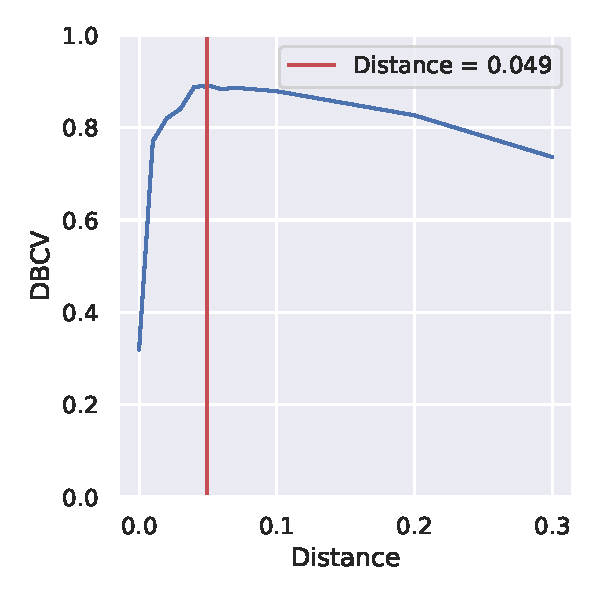
\includegraphics[width=\dimexpr\textwidth-2\fboxsep-2\fboxrule,page=1]{UMAP/Cluster_DBCV_Segment_4.pdf}}
\end{figure}

\begin{table}[!hbt]
    \pgfplotstabletypeset[
        every head row/.style={
            before row={
                \toprule
                & \multicolumn{3}{l}{\textbf{Cluster}} &  & \multicolumn{2}{l}{\textbf{mixed}} &\\
                \cmidrule(lr){2-4}\cmidrule(lr){6-7}
            },
            after row={
                \midrule
            },
        },
        every last row/.style={
            after row={
                %... & ... & ... & ... & ... & ... & ... & ...\\
                \bottomrule
            },
        },
        begin table=\begin{tabular*}{\textwidth},
        end table=\end{tabular*},
        header=false,
        skip first n=1,
        columns={0,1,2,3,4,5,6,7},
        columns/0/.style={multicolumn names=l,column name=\textbf{Segment}, column type=@{\extracolsep{\fill} }r},
        columns/1/.style={multicolumn names=l,column name=\textbf{\#Final}, column type=r},
        columns/2/.style={multicolumn names=l,column name=\textbf{\#Raw}, column type=r},
        columns/3/.style={multicolumn names=l,column name=\textbf{Normalized}, column type=r},
        columns/4/.style={multicolumn names=l,column name=\textbf{\#Unclustered}, column type=r},
        columns/5/.style={multicolumn names=l,column name=\textbf{H}, column type=r},
        columns/6/.style={multicolumn names=l,column name=\textbf{N}, column type=r},
        columns/7/.style={multicolumn names=l,column name=\bm{$\varepsilon$}, column type=r},
        %row predicate/.code={%
        %    \ifnum#1>0\relax
        %        \ifnum#1<2\relax
        %            \pgfplotstableuserowfalse
        %        \fi
        %    \fi
        %}
    ]
    {UMAP/information.csv}
    \caption[A table]{\textbf{A table.} A table.}
    \label{tab:3.1}
\end{table}

\blindtext